\section{Recursion and marginals}\label{sec:marginals}
In this section, we analyze the marginal bounds on the set of edges adjacent to a given vertex in a $\beta$-extra list-edge-coloring instance under various conditions.
\subsection{Marginal bounds for general edge coloring}
We begin by examining the marginal bounds on general graphs.
%edge coloring instances, which provides a fundamental understanding of the behavior of these bounds on any graphs.
\begin{lemma}\label{lem:claw-marginal-generalized}
     Given a list-edge-coloring instance $(G, \+L)$ where $G=(V, E)$,
     and a vertex $v\in V$ such that $\forall e\in E_{v}: \abs{\+L(v)}-\deg(e) \ge \beta\ge 2$.
    Then for any $v\in V$, $F\subseteq E(v)$ and color $a$:
    \[\Pr[G,\+L]{a\in c(F)} \le \frac{|F|}{\beta - 1 + |F|}\quad\mbox{and}\quad \frac{\Pr[G,\+L]{a\in c(F)}}{\Pr[G,\+L]{a \notin c(E(v))}} \le \frac{|F|}{\beta - 1}.\]
\end{lemma}
\begin{proof}
We denote the set of all proper colorings on $(G, \+L)$ by $\Omega$, and define
\[A \defeq \set{\omega\in \Omega \mid \exists e\in F: \omega(e) = a}.\]
Then define a function $\iota: (\Omega\setminus A)\times A\to \mathbb R_{\ge 0} $ such that for any $\omega'\in A$:
\begin{equation}\label{eq:marginal-sum-is-1}
\sum_{\omega\in \Omega\setminus A} \iota(\omega, \omega') = 1.
\end{equation}
To continue with the construction of $\iota$, for any $\omega' \in A$:
\[
    B(\omega')\defeq \set{\omega\in \Omega\setminus A : d(\omega, \omega') = 1}.
\]
where $d$ is the Hamming distance, i.e., the number of edges colored differently between the two colorings.
Then
\begin{align*}
\iota(\omega, \omega') \defeq
\begin{cases}
\frac{1}{|B(\omega')|},& \omega\in B(\omega')\\
0, &\text{otherwise}
\end{cases}.
\end{align*}
It is easy to verify \cref{eq:marginal-sum-is-1} holds.
Notice that if $\omega\in B(\omega')$ such that $\omega'(e) = a$ for some $e\in F$,
then $\omega$ is obtained from $\omega'$ by recoloring $e$ to another color other than $a$. 
There are at least $\beta-1$ choices according to the assumption, so $|B(\omega')|\ge \beta-1$ for any $\omega'\in A$.

Similarly, if $\omega'\in B(\omega)$, then $\omega'$ is obtained from $\omega$ by recoloring an edge $e\in F$ to $a$,
there are at most $|F|$ choices,
so we have $\sum_{\omega'} \iota(\omega, \omega') \le \frac{|F|}{\beta-1}$ for all $\omega\in \Omega\setminus A$.

Then
\begin{align*}
\Pr[G,\+L]{a\in c(F)}
&= \frac{\sum_{\omega'\in A}1}{\sum_{\omega\in \Omega\setminus A} 1 + \sum_{\omega'\in A}1}\\
&= \frac{\sum_{\omega'\in A}\sum_{\omega\in \Omega\setminus A} \iota(\omega, \omega')}
        {\sum_{\omega\in \Omega\setminus A} 1 + \sum_{\omega'\in A}\sum_{\omega\in \Omega\setminus A} \iota(\omega, \omega')}\\
&= \frac{\sum_{\omega\in \Omega\setminus A} \sum_{\omega'\in A} \iota(\omega, \omega')}
        {\sum_{\omega\in \Omega\setminus A} \left(1 + \sum_{\omega'\in A}\iota(\omega, \omega')\right)}\\
&\le \frac{|F|/(\beta-1)}{1 + |F|/(\beta-1)} = \frac{|F|}{\beta-1+|F|},
\end{align*}
proving the first part of the lemma.

Similarly, we define $\Omega_0\defeq\set{\omega\in \Omega \mid \not\exists e\in E(v) : \omega(e) = a}$.
Note that by definition, $\iota(\cdot, \cdot)$ is supported on $\Omega\times A$, so we have
\begin{align*}
\frac{\Pr[G,\+L]{a\in c(F)}}{\Pr[G,\+L]{a\notin c(E(v))}}
&= \frac{\sum_{\omega'\in A}1}{\sum_{\omega\in \Omega_0} 1}\\
&= \frac{\sum_{\omega'\in A}\sum_{\omega\in \Omega\setminus A} \iota(\omega, \omega')}
        {\sum_{\omega\in \Omega_0} 1 }\\
% &= \frac{\sum_{\omega'\in A}\sum_{\omega\in \Omega_0} \iota(\omega, \omega')}
%         {\sum_{\omega\in \Omega_0} 1 }\\
&= \frac{\sum_{\omega\in \Omega_0} \sum_{\omega'\in A} \iota(\omega, \omega')}
        {\sum_{\omega\in \Omega_0} 1}\\
&\le \frac{|F|}{\beta-1}.
\end{align*}
\end{proof}

Especially, when $\abs{F}=1$, we have the following corollary.
\begin{corollary}\label{cor:marginal-bound-gamma-delta}
    Let $(G=(V, E), \+L)$ be a $\beta$-extra list-edge-coloring instance. Then for any $e\in E, v\in V, a\in \+L(e)$, 
    \[
    \frac{\Pr[G,\+L]{c(e)=a}}{\Pr[G,\+L]{a\notin c(E_v)}} \le \frac{1}{\beta-1}.
    \]
\end{corollary}

\subsection{Tree recursion for edge coloring}\label{sec:recursion}
We now turn our attention to a more specialized structure: trees. Throughout this section, we fix a $\beta$-extra edge-coloring instance $(T=(V,E),\+{L})$ with root $r$. For any vertex $v \in V$, let $T_v$ be the sub-tree of $T$ rooted at $v$ and $E_{T_v}$ be the edge set of $T_v$. Let $C_v$ be the set of proper partial colorings on $E_{T_v}(v)$ and $\+D(C_v)$ be the set of all distributions on $C_v$. 

Assume $r$ has $d$ children $v_1, v_2, \dots, v_d$. For any $i\in [d]$, let $e_i = (r, v_i)$ and $T_i = T_{v_i}$. For brevity, since the color lists are fixed, we omit the color lists $\+L$ in the subscript in $\Pr[T,\+L]{\cdot}$ and $Z_{T,\+L}(\cdot)$. For any $i\in [d]$, we also write $\Pr[T_i]{\cdot}$ for $\Pr[T_i, \+L|_{T_i}]{\cdot}$ and $Z_{T_i}(\cdot)$ for $Z_{T_i,\+L|_{T_i}}(\cdot)$.

We introduce a tree recursion on the marginal distributions of partial colorings on ``brooms'', where a ``broom'' is referred to as the edge set $E_{T_v}(v)$ for a vertex $v\in V$. This recursion demonstrates how the marginal distributions on brooms propagate through the tree structure as in \Cref{fig:broom-recursion}.
%\ctodo{The notations $\Pr[T]{\cdot}, \Pr[T_i]{}$ are not defined.}
%\yltodo{Added an introduction to broom and the figure}
\usetikzlibrary{trees}
    \tikzset{
        arn/.style = {circle, draw=black, fill=white, thick},
}
\begin{figure}[H]
\centering
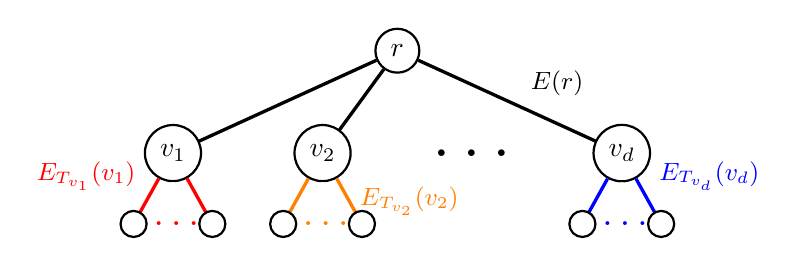
\begin{tikzpicture}
    [sibling distance = 1.9cm,level distance = 1.3cm] \node [arn] {$r$}
    child[edge from parent/.style={very thick,draw}] {
        [sibling distance = 0.5cm,level distance = 0.9cm]node [arn] {$v_1$}
        child {
            [red] node [arn] {}
            edge from parent node[above left] {\small $E_{T_{v_1}}(v_1)$}
        }
        child {[white] node [red] {\tiny$\ $\Large$\dots$} }
        child {[red] node [arn] {} }
    }
    child[edge from parent/.style={very thick,draw}] {
        [sibling distance = 0.5cm,level distance = 0.9cm]node [arn] {$v_2$}
        child {[orange] node [arn] {}}
        child {[white] node [orange] {\tiny$\ $\Large$\dots$} }
        child {
            [orange] node [arn] {}
            edge from parent node[right] {\small $E_{T_{v_2}}(v_2)$}
        }
    }
    child[edge from parent/.style={very thick,draw}] {
        [white] node [black] {\Huge$\dots$}
    }
    child[edge from parent/.style={very thick,draw}] {
        [sibling distance = 0.5cm,level distance = 0.9cm]node [arn] {$v_d$}
        child {[blue] node [arn] {}}
        child {[white] node [blue] {\tiny$\ $\Large$\dots$} }
        child {
            [blue] node [arn] {}
            edge from parent node[above right] {\small $E_{T_{v_d}}(v_d)$}
        }
        edge from parent node[above right] {\small $E(r)$}
    };
\end{tikzpicture}
\caption{Brooms on a tree}
\label{fig:broom-recursion}
\end{figure}

\begin{lemma}\label{lem:tree-recursion}
    Given distributions $\*{p}_i=\tp{\Pr[T_i]{c(E_{T_i}(v_i))=\tau}}_{\tau\in C_{v_i}}$ on $C_{v_i}$ for each $v_i$, we can compute the marginal distribution $\*{p}_r=\tp{\Pr[T]{c(E(r))=\pi}}_{\pi \in C_r}$ on $C_r$:
\begin{align*}
    \*p_r(\pi)=f_\pi(\set{\*{p}_i}_{i\in [d]})=\frac{\prod_i \sum_{\tau
    \in C_{v_i}: \pi(e_i)\notin \tau} \*p_{i}(\tau)}{\sum_{\rho \in C_r} \prod_i \sum_{\tau
    \in C_{v_i}: \rho(e_i)\notin \tau} \*p_{i}(\tau)}.
\end{align*}
\end{lemma}
\begin{proof}
    By the definition of marginal probabilities, we have
\begin{align*}
    \*p_r(\pi)&=\Pr[T]{c(E(r))=\pi}\\
    &=\frac{Z_T(c(E(r))=\pi)}{\sum_{\rho \in C_r} Z_T(c(E(r))=\rho)}.
\end{align*}
Since $T$ is a tree, we can further write 
\begin{align*}
    \*p_r(\pi)&=\frac{\prod_i Z_{T_i}(\pi(e_i)\not\in c(E_{T_i}(v_i)))}{\sum_{\rho \in C_r} \prod_i Z_{T_i}(\rho(e_i)\not\in c(E(v_i)))}\\
    &=\frac{\prod_i \sum_{\tau
    \in C_{v_i} : \pi(e_i)\notin \tau} Z_{T_i}(c(E_{T_i}(v_i))=\tau)}{\sum_{\rho \in C_r} \prod_i \sum_{\tau
    \in C_{v_i}: \rho(e_i)\notin \tau} Z_{T_i}(c(E_{T_i}(v_i))=\tau)}\\
    &=\frac{\prod_i \sum_{\tau
    \in C_{v_i}: \pi(e_i)\notin \tau} \Pr[T_i]{c(E_{T_i}(v_i))=\tau}}{\sum_{\rho \in C_r} \prod_i \sum_{\tau
    \in C_{v_i}: \rho(e_i)\notin \tau} \Pr[T_i]{c(E_{T_i}(v_i))=\tau}}.
\end{align*}
\end{proof}
We will regard $f=(f_\pi)_{\pi \in C_r}: \bb{R}_{\geq 0}^{C_{v_1}}\times \bb{R}_{\geq 0}^{C_{v_2}}\times \cdots \times \bb{R}_{\geq 0}^{C_{v_d}} \rightarrow \+D(C_{r})$ as a function taking inputs $\*p = (\*p_1, \*p_2, \dots, \*p_d)$ where $\*p_i\in \bb R_{\ge 0}^{C_{v_i}}$ for $i\in [d]$. Note that in some cases, $\*p$ might not encode a distribution.

\subsection{Marginal bounds propagated by recursion}\label{sec:marginal_bounds_on_trees}
Now we can give marginal bounds of probabilities that propagated by the recursion. For brevity, we define some notations of marginals for any non-zero vector $\*p_v\in \bb{R}_{\geq 0}^{C_v}$ with $v\in V$: Let $\*p_v(c)=\sum_{\tau \in C_v:c \in \tau} \*p_v(\tau)$, $\*p_v(\bar{c})=\sum_{\tau \in C_v:a \notin \tau} \*p_v(\tau)$, and $\*p_v(\bar{c_1},\bar{c_2})=\sum_{\tau \in C_v:c_1,c_2 \notin \tau} \*p_v(\tau)$.
Especially, for $\*p_r \in \+D(C_r)$, we define $\*p_r(i,c)=\sum_{\pi \in C_r: \pi(e_i)=c} \*p_r(\pi)$, and $\*p_r(i,c_1,j,c_2)=\sum_{\pi \in C_r: \pi(e_i)=c_1, \pi(e_j)=c_2} \*p_r(\pi)$.

By \Cref{lem:tree-recursion}, we have
\begin{equation}\label{eq:tree-recursion-short}
    \*p_r(\pi)=f_\pi(\set{\*{p}_i}_{i\in [d]})=
    \frac{\prod_i \*p_{v_i}(\ol{\pi(e_i)})}
    {\sum_{\rho \in C_r} \prod_i \*p_{v_i}(\ol{\rho(e_i)})}.
\end{equation}

We have the following lemma similar to \Cref{lem:claw-marginal-generalized}
on trees. Note that we do not require $\*p_i$'s to be distributions in \Cref{lem:marginal_bound_1}.
\begin{lemma}\label{lem:marginal_bound_1}
     Given non-zero vector $\*p_i\in \bb{R}_{\geq 0}^{C_{v_i}}$ for each $i\in [d]$ and $\*p_r = f(\{\*p_i\}_{i\in[d]})$, we have that for any color $a \in [q]$,
    \[
        \*p_r(a) \leq \frac{d}{\beta - 1 + d} \quad\mbox{and}\quad  \frac{\*p_r(a)}{\*p_r(\overline{a})} \leq \frac{d}{\beta - 1}.
    \]
    \end{lemma}
    \begin{proof}[Proof of \Cref{lem:marginal_bound_1}] The proof is similar to that of \Cref{lem:claw-marginal-generalized}.
    Define
\[A \defeq \set{\omega\in \Omega \mid \exists e\in E(r): \omega(e) = a}.\]
For any $\omega' \in A$, define
\[
    B(\omega')\defeq \set{\omega\in C_r\setminus A : d(\omega, \omega') = 1}.
\]
where $d$ is the Hamming distance, i.e., the number of edges colored differently between the two colorings.
        We define
        $$
            \iota(\omega,\omega') := \begin{cases}
                \frac{w(\omega)}{\sum_{\omega\in B(\omega')}w(\omega)}w(\omega'),&\omega\in B(\omega')
                \\ 0,& \text{otherwise}
            \end{cases}
        $$
        where $w(\omega) \defeq \prod_{i=1}^{d} \*p_i(\overline{\omega(e_i)})$. Note that $\sum_{\omega \in C_r\setminus A} \iota(\omega,\omega')=w(\omega')$.
        For any $\omega' \in A$, assuming $\omega'(e_i) = a$, by~\eqref{eq:tree-recursion-short},
        \begin{align*}
            \frac{w(\omega')}{\sum_{\omega\in B(\omega')} w(\omega)}
              &= \frac{\*p_i(\overline a)}{\sum_{a'\neq a} \*p_i(\overline{a'})}
            \\&= \frac{\sum_{\tau\in C_{v_i},a\notin \tau}\*p_i(\tau)}
              {\sum_{\tau\in C_{v_i}} \tp{\sum_{a'\neq a}\1{a\notin \tau}} \*p_i(\tau)}
            \\&\leq \frac{\sum_{\tau\in C_{v_i},a\notin \tau}\*p_i(\tau)}
              {\sum_{\tau\in C_{v_i}, a\notin\tau} \tp{\sum_{a'\neq a}\1{a\notin \tau}} \*p_i(\tau)}
            \\&\le \frac{1}{\beta-1}.
        \end{align*}
    The last inequality is because $\sum_{a'\neq a}\1{a\notin \tau}\ge \beta-1$ for all $\tau\in C_{v_i}$.
    Then we have $\sum_{\omega' \in A} \iota(\omega, \omega')\leq \frac{d}{\beta-1} w(\omega)$.    
    Therefore by~\eqref{eq:tree-recursion-short},
    \begin{align*}
\*p_r(a)
&= \frac{\sum_{\omega'\in A} w(\omega')}{\sum_{\omega\in C_r\setminus A} w(\omega) + \sum_{\omega'\in A} w(\omega')}\\
&= \frac{\sum_{\omega'\in A}\sum_{\omega\in C_r\setminus A} \iota(\omega, \omega')}
        {\sum_{\omega\in \Omega\setminus A} w(\omega) + \sum_{\omega'\in A}\sum_{\omega\in C_r\setminus A} \iota(\omega, \omega')}\\
&= \frac{\sum_{\omega\in C_r\setminus A} \sum_{\omega'\in A} \iota(\omega, \omega')}
        {\sum_{\omega\in C_r\setminus A} \left(w(\omega) + \sum_{\omega'\in A}\iota(\omega, \omega')\right)}\\
&\le \frac{d/(\beta-1)}{1 + d/(\beta-1)} = \frac{d}{\beta-1+d}.
\end{align*}
Similarly,
\begin{align*}
\frac{\*p_r(a)}{\*p_r(\bar{a})}
&= \frac{\sum_{\omega'\in A} w(\omega')}{\sum_{\omega\in C_r\setminus A} w(\omega)}
= \frac{\sum_{\omega'\in A}\sum_{\omega\in C_r\setminus A} \iota(\omega, \omega')}
        {\sum_{\omega\in \Omega\setminus A} w(\omega)}
\le \frac{d}{\beta-1}.
\end{align*}
    \end{proof}
    
\begin{lemma}\label{lem:marginal_bound_2}
    Given non-zero vector $\*p_i\in \bb{R}_{\geq 0}^{C_{v_i}}$ for each $i\in [d]$ and $\*p_r = f(\{\*p_i\}_{i\in[d]})$, we have that for any color $a\in [q]$ and $j\in [d]$,
    $$
        \*p_r(j,a) \leq \frac{\*p_j(\overline a)}{(\beta - 1)\sum_{\tau\in C_{v_j}}\*p_j(\tau)}.
    $$
\end{lemma}
\begin{proof}
        We have that
        \begin{align*}
            \*p_r(j,a) &= \frac{\displaystyle \sum_{\substack{\sigma\text{: coloring on }E(v)\setminus e_j\\a\notin \sigma}} \prod_{i\neq j}\*p_i(\overline{\sigma(v_i)})\*p_j(\overline{a})}{\displaystyle \sum_{\sigma\text{: coloring on }E(r)\setminus e_j} \prod_{i\neq j}\*p_i(\overline{\sigma(v_i)})(\sum_{a'\notin \sigma} \*p_j(\overline{a'}))}
            \\&\leq \sup_{\sigma}\frac{\displaystyle \*p_j(\overline{a})}{\displaystyle \sum_{a'\notin \sigma} \*p_j(\overline{a'})}
            \\&= \sup_{\sigma}\frac{\displaystyle \*p_j(\overline{a})}{\displaystyle(\+L(e_j) - \deg(v_j) + 1)\sum_{\tau\in C_{v_j}}\*p_j(\tau) - \sum_{a'\in \sigma} \*p_j(\overline{a'})}
            \\&\leq \frac{\*p_j(\overline{a})/(\sum_{\tau\in C_{v_j}}\*p_j(\tau))}{\+L(e_j) - \deg(v_j) - \deg(r) + 1}.
        \end{align*}
\end{proof}
